\documentclass[11pt,a4paper]{article}

\usepackage[top=20mm,bottom=26mm,left=20mm,right=20mm,headheight=15pt,footskip=12mm]{geometry}

\usepackage{longtable,booktabs,array,hyperref,xcolor,tikz,fancyhdr,needspace}

\usepackage{fontspec,xeCJK}

\setmainfont[Ligatures=TeXOff]{Times New Roman}

\setsansfont[Ligatures=TeXOff]{Times New Roman}

\setmonofont[Ligatures=TeXOff,WordSpace={1,1,1}]{Times New Roman}

\setCJKmainfont{Noto Serif CJK SC}

\setCJKsansfont{Noto Serif CJK SC}

\setCJKmonofont{Noto Serif CJK SC}

\newfontfamily\vulcanmathsymbols{Noto Serif CJK SC}

\XeTeXgenerateactualtext=1

\definecolor{vulcan}{HTML}{BB3E23}

\definecolor{vulcanblue}{HTML}{1B4F72}

\renewcommand{\thesection}{\Roman{section}}

\renewcommand{\thesubsection}{\Alph{subsection}}

\pgfdeclarelayer{connections}\pgfdeclarelayer{edge labels}\pgfsetlayers{connections,main,edge labels}

\hypersetup{hidelinks}

\newcolumntype{L}[1]{>{\raggedright\arraybackslash\hspace{0pt}}p{#1}}

\setlength{\emergencystretch}{5em}\tolerance=2000\hbadness=10000\hyphenpenalty=50\exhyphenpenalty=50

\setlength{\parindent}{0pt}\setlength{\parskip}{5pt}

\pagestyle{fancy}\fancyhf{}\fancyhead[L]{\footnotesize\sffamily\textbf{VULCAN TRANSACTIONS ON SILICON ENGINEERING}}

\fancyhead[R]{\footnotesize\sffamily RTL Microarchitecture \& Silicon Signoff}\fancyfoot[C]{\footnotesize\sffamily Page \thepage}

\begin{document}

{\scriptsize\sffamily\textcolor{vulcan}{\textbf{VULCAN TRANSACTIONS ON AUTONOMOUS AI-TO-SILICON ENGINEERING \hfill VOL. 2026 \textperiodcentered{} ARCHITECTURAL SIGNOFF PAPER}}\par}

\vspace{1pt}\textcolor{vulcan}{\rule{\textwidth}{1.2pt}}\vspace{4pt}

\begin{center}

{\sffamily\LARGE\bfseries BILLET-F2: Four-Channel Fixed-Point FIR RTL IP\par}\vspace{3pt}

{\small\sffamily\textbf{Sufeng Guo (\allowbreak{}sufeng\_\allowbreak{}guo@smail.nju.edu.cn)\allowbreak{}} \textperiodcentered{} Microsoft Research Asia \textperiodcentered{} Technical Design and Verification Report\par}\vspace{1pt}

{\scriptsize\sffamily\textcolor{black!75}{Silicon Platform: Intel Arria 10 GX (\texttt{10AX115N3F40E2SG}) PCIe Gen3x8 \textperiodcentered{} Toolchain: Icarus Verilog 12.0 / Yosys 0.33 / Quartus Prime 17.1 STA \textperiodcentered{} 24 October 2026 (\allowbreak{}2026-10-24 20:14 UTC+\allowbreak{}8 Beijing Time)\allowbreak{}}\par}

\end{center}\vspace{2pt}

\renewcommand{\abstractname}{\textcolor{vulcanblue}{Abstract}}\begin{abstract}\noindent BILLET-F2 implements four independently configured FIR channels around one shared,\allowbreak{} configurable parallel multiply-accumulate engine. It provides independent sample histories,\allowbreak{} per-channel double-buffered coefficients and atomic bank swaps,\allowbreak{} while preserving BILLET-F1 channel-zero numerical and cycle behavior with one MAC lane. The mandatory behavioral matrix covered all 15 legal parameter combinations at seeds 17,\allowbreak{} 89 and 233: 102,\allowbreak{}339 retired samples matched an independent integer convolution model with zero output-code error. Fifteen additional F1 compatibility runs compared 8,\allowbreak{}472 retirements with zero differences. Reset canceled 90 and 30 transactions respectively; these were accounted separately from compared outputs. Three semantic mutants were detected,\allowbreak{} and all 15 configurations passed generic synthesis and latch checks. These results establish simulated digital behavior and generic synthesizability,\allowbreak{} not physical performance. [\allowbreak{}E019–E022]\allowbreak{}\par\vspace{2pt}{\scriptsize\textbf{\textcolor{vulcanblue}{Index Terms---}}Autonomous RTL Generation, SystemVerilog, Intel Arria 10 GX FPGA, TimeQuest 100~MHz+ Timing Closure, PCIe Gen3x8 Hardware-in-the-Loop (HIL), Bit-Exact Fixed-Point Verification.}\end{abstract}\vspace{2pt}

\needspace{5\baselineskip}\section{Architecture and design rationale}

The design uses one globally shared computation engine,\allowbreak{} no input queue and one output register. Separate histories and coefficient banks isolate channel state without duplicating the entire datapath. Each computation captures its channel and active-bank identity; global commit exclusion preserves that ownership through output retirement. This conservative policy retains F1 control semantics but prevents unrelated channels from committing while the engine or output is occupied. Parallel lanes process consecutive taps,\allowbreak{} with a balanced full-width reduction tree and combinational final rounding. The five synthesizable modules total 13,\allowbreak{}997 bytes and 368 source lines. [\allowbreak{}E001,\allowbreak{} E003–E007,\allowbreak{} E022]\allowbreak{}

\begin{center}\begin{minipage}{\textwidth}\centering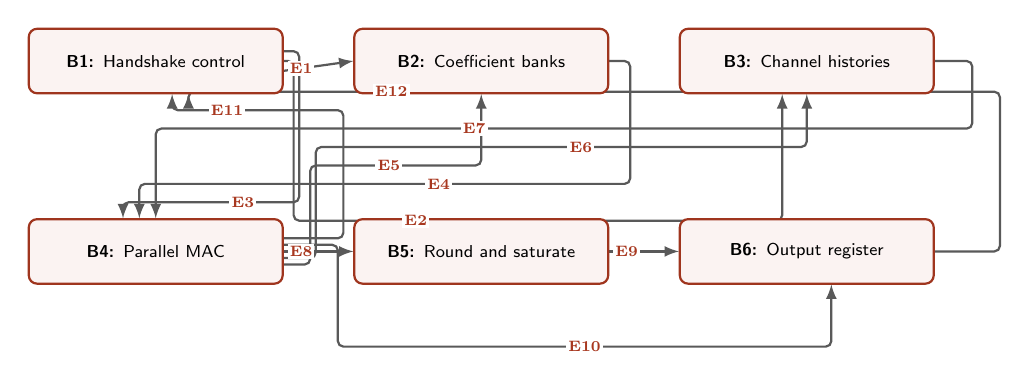
\begin{tikzpicture}[scale=0.78,transform shape,every node/.style={font=\footnotesize\sffamily},>=latex]

\node[draw=vulcan!85!black,thick,rounded corners=3pt,fill=vulcan!6,text width=3.9cm,minimum height=1.05cm,align=center] (b0) at (0.0,0.0) {\textbf{B1:} Handshake control};

\node[draw=vulcan!85!black,thick,rounded corners=3pt,fill=vulcan!6,text width=3.9cm,minimum height=1.05cm,align=center] (b1) at (5.3,0.0) {\textbf{B2:} Coefficient banks};

\node[draw=vulcan!85!black,thick,rounded corners=3pt,fill=vulcan!6,text width=3.9cm,minimum height=1.05cm,align=center] (b2) at (10.6,0.0) {\textbf{B3:} Channel histories};

\node[draw=vulcan!85!black,thick,rounded corners=3pt,fill=vulcan!6,text width=3.9cm,minimum height=1.05cm,align=center] (b3) at (0.0,-3.1) {\textbf{B4:} Parallel MAC};

\node[draw=vulcan!85!black,thick,rounded corners=3pt,fill=vulcan!6,text width=3.9cm,minimum height=1.05cm,align=center] (b4) at (5.3,-3.1) {\textbf{B5:} Round and saturate};

\node[draw=vulcan!85!black,thick,rounded corners=3pt,fill=vulcan!6,text width=3.9cm,minimum height=1.05cm,align=center] (b5) at (10.6,-3.1) {\textbf{B6:} Output register};

\begin{pgfonlayer}{connections}

\draw[->,thick,black!65] ([yshift=-0.160cm]b0.east) -- coordinate[pos=0.25] (e0) ([yshift=0.000cm]b1.west);

\draw[->,thick,black!65,rounded corners=2pt] ([yshift=0.000cm]b0.east) -- (2.245,0.000) -- (2.245,-2.600) -- coordinate[pos=0.25] (e1) (10.200,-2.600) -- ([xshift=-0.400cm]b2.south);

\draw[->,thick,black!65,rounded corners=2pt] ([yshift=0.160cm]b0.east) -- (2.335,0.160) -- (2.335,-2.300) -- coordinate[pos=0.32] (e2) (-0.533,-2.300) -- ([xshift=-0.533cm]b3.north);

\draw[->,thick,black!65,rounded corners=2pt] ([yshift=0.000cm]b1.east) -- (7.725,0.000) -- (7.725,-2.000) -- coordinate[pos=0.39] (e3) (-0.267,-2.000) -- ([xshift=-0.267cm]b3.north);

\draw[->,thick,black!65,rounded corners=2pt] ([yshift=-0.213cm]b3.east) -- (2.515,-3.313) -- (2.515,-1.700) -- coordinate[pos=0.46] (e4) (5.300,-1.700) -- ([xshift=0.000cm]b1.south);

\draw[->,thick,black!65,rounded corners=2pt] ([yshift=-0.107cm]b3.east) -- (2.605,-3.207) -- (2.605,-1.400) -- coordinate[pos=0.54] (e5) (10.600,-1.400) -- ([xshift=0.000cm]b2.south);

\draw[->,thick,black!65,rounded corners=2pt] ([yshift=0.000cm]b2.east) -- (13.295,0.000) -- (13.295,-1.100) -- coordinate[pos=0.61] (e6) (0.000,-1.100) -- ([xshift=0.000cm]b3.north);

\draw[->,thick,black!65] ([yshift=0.000cm]b3.east) -- coordinate[pos=0.25] (e7) ([yshift=0.000cm]b4.west);

\draw[->,thick,black!65] ([yshift=0.000cm]b4.east) -- coordinate[pos=0.25] (e8) ([yshift=0.000cm]b5.west);

\draw[->,thick,black!65,rounded corners=2pt] ([yshift=0.107cm]b3.east) -- (2.965,-2.993) -- (2.965,-4.650) -- coordinate[pos=0.50] (e9) (11.000,-4.650) -- ([xshift=0.400cm]b5.south);

\draw[->,thick,black!65,rounded corners=2pt] ([yshift=0.213cm]b3.east) -- (3.055,-2.887) -- (3.055,-0.800) -- coordinate[pos=0.68] (e10) (0.267,-0.800) -- ([xshift=0.267cm]b0.south);

\draw[->,thick,black!65,rounded corners=2pt] ([yshift=0.000cm]b5.east) -- (13.745,-3.100) -- (13.745,-0.500) -- coordinate[pos=0.75] (e11) (0.533,-0.500) -- ([xshift=0.533cm]b0.south);

\end{pgfonlayer}

\begin{pgfonlayer}{edge labels}

\node[fill=white,inner sep=1pt,font=\scriptsize\bfseries,text=vulcan!90!black] at (e0) {E1};

\node[fill=white,inner sep=1pt,font=\scriptsize\bfseries,text=vulcan!90!black] at (e1) {E2};

\node[fill=white,inner sep=1pt,font=\scriptsize\bfseries,text=vulcan!90!black] at (e2) {E3};

\node[fill=white,inner sep=1pt,font=\scriptsize\bfseries,text=vulcan!90!black] at (e3) {E4};

\node[fill=white,inner sep=1pt,font=\scriptsize\bfseries,text=vulcan!90!black] at (e4) {E5};

\node[fill=white,inner sep=1pt,font=\scriptsize\bfseries,text=vulcan!90!black] at (e5) {E6};

\node[fill=white,inner sep=1pt,font=\scriptsize\bfseries,text=vulcan!90!black] at (e6) {E7};

\node[fill=white,inner sep=1pt,font=\scriptsize\bfseries,text=vulcan!90!black] at (e7) {E8};

\node[fill=white,inner sep=1pt,font=\scriptsize\bfseries,text=vulcan!90!black] at (e8) {E9};

\node[fill=white,inner sep=1pt,font=\scriptsize\bfseries,text=vulcan!90!black] at (e9) {E10};

\node[fill=white,inner sep=1pt,font=\scriptsize\bfseries,text=vulcan!90!black] at (e10) {E11};

\node[fill=white,inner sep=1pt,font=\scriptsize\bfseries,text=vulcan!90!black] at (e11) {E12};

\end{pgfonlayer}

\end{tikzpicture}\par\vspace{3pt}

{\small\textbf{Figure 1:} Top-level microarchitectural functional block map and directed inter-module bus topology.}\end{minipage}\end{center}

{\small\renewcommand{\arraystretch}{1.18}\begin{longtable}{@{}L{0.24\textwidth}|L{0.7\textwidth}@{}}\toprule

\textbf{Block} & \textbf{Responsibility}\\\midrule\endhead

B1: Handshake control & Control logic in billet\_\allowbreak{}f2\_\allowbreak{}top determines sample,\allowbreak{} configuration and commit acceptance,\allowbreak{} enforces commit priority and excludes swaps during computation or valid output.\\[2pt]\hline

B2: Coefficient banks & billet\_\allowbreak{}f2\_\allowbreak{}coeff\_\allowbreak{}bank,\allowbreak{} instance u\_\allowbreak{}coeff\_\allowbreak{}bank,\allowbreak{} owns four independent bank pairs,\allowbreak{} active selectors and fresh-write masks. Parallel reads select the captured channel and bank.\\[2pt]\hline

B3: Channel histories & billet\_\allowbreak{}f2\_\allowbreak{}history,\allowbreak{} instance u\_\allowbreak{}history,\allowbreak{} owns four delay lines. Only the accepted sample's channel shifts; tap zero becomes the newest sample.\\[2pt]\hline

B4: Parallel MAC & billet\_\allowbreak{}f2\_\allowbreak{}mac,\allowbreak{} instance u\_\allowbreak{}mac,\allowbreak{} captures ownership and tracks tap groups. Signed 16-by-16 products are extended before balanced reduction and exact accumulation.\\[2pt]\hline

B5: Round and saturate & billet\_\allowbreak{}f2\_\allowbreak{}round\_\allowbreak{}sat,\allowbreak{} instance u\_\allowbreak{}round\_\allowbreak{}sat,\allowbreak{} combinationally converts the exact final sum to signed Q1.15 using nearest-even rounding and saturation.\\[2pt]\hline

B6: Output register & Registers in billet\_\allowbreak{}f2\_\allowbreak{}top capture the final result and channel,\allowbreak{} hold them under backpressure and permit retirement alongside a replacement input.\\[2pt]\hline

\bottomrule\end{longtable}}

{\small\renewcommand{\arraystretch}{1.18}\begin{longtable}{@{}L{0.24\textwidth}|L{0.7\textwidth}@{}}\toprule

\textbf{Directed relationship} & \textbf{Meaning}\\\midrule\endhead

E1: B1 to B2 & Accepted coefficient writes and commits\\[2pt]\hline

E2: B1 to B3 & Accepted sample,\allowbreak{} channel and history push\\[2pt]\hline

E3: B1 to B4 & Start and accepted transaction identity\\[2pt]\hline

E4: B2 to B4 & Active-bank identity and coefficient operands\\[2pt]\hline

E5: B4 to B2 & Captured channel,\allowbreak{} bank and tap-group address\\[2pt]\hline

E6: B4 to B3 & Captured channel and tap-group address\\[2pt]\hline

E7: B3 to B4 & Parallel history operands\\[2pt]\hline

E8: B4 to B5 & Exact final accumulator sum\\[2pt]\hline

E9: B5 to B6 & Rounded,\allowbreak{} saturated result\\[2pt]\hline

E10: B4 to B6 & Final capture enable and channel\\[2pt]\hline

E11: B4 to B1 & Computation busy\\[2pt]\hline

E12: B6 to B1 & Output occupancy\\[2pt]\hline

\bottomrule\end{longtable}}

\needspace{9\baselineskip}\section{Interfaces and configuration}

{\small\renewcommand{\arraystretch}{1.18}\begin{longtable}{@{}L{0.21\textwidth}|L{0.12\textwidth}|L{0.12\textwidth}|L{0.45\textwidth}@{}}\toprule

\textbf{Signal /\allowbreak{} group} & \textbf{Direction} & \textbf{Width} & \textbf{Contract}\\\midrule\endhead

clk,\allowbreak{} rst\_\allowbreak{}n & Input & 1 bit each & Rising-edge clock and active-low asynchronous reset. Transactions use pre-edge valid/\allowbreak{}ready values.\\[2pt]\hline

s\_\allowbreak{}data,\allowbreak{} s\_\allowbreak{}channel,\allowbreak{} s\_\allowbreak{}valid; s\_\allowbreak{}ready & Input; output & Signed 16,\allowbreak{} 2,\allowbreak{} 1; 1 bits & Input sample stream. Channel encodings 0–3 are legal. Producers hold valid,\allowbreak{} data and channel while stalled.\\[2pt]\hline

m\_\allowbreak{}data,\allowbreak{} m\_\allowbreak{}channel,\allowbreak{} m\_\allowbreak{}valid; m\_\allowbreak{}ready & Output; input & Signed 16,\allowbreak{} 2,\allowbreak{} 1; 1 bits & Ordered result stream. Valid data and channel remain stable until retirement or reset. Data and channel are zero whenever m\_\allowbreak{}valid is low.\\[2pt]\hline

cfg\_\allowbreak{}valid,\allowbreak{} cfg\_\allowbreak{}channel,\allowbreak{} cfg\_\allowbreak{}addr,\allowbreak{} cfg\_\allowbreak{}data; cfg\_\allowbreak{}ready & Input; output & 1,\allowbreak{} 2,\allowbreak{} ADDR\_\allowbreak{}W,\allowbreak{} signed 16; 1 bits & Writes the addressed channel's inactive coefficient bank. Acceptance requires a legal address and no commit request. Address one is rejected even at TAP\_\allowbreak{}COUNT=\allowbreak{}1.\\[2pt]\hline

commit\_\allowbreak{}valid,\allowbreak{} commit\_\allowbreak{}channel; commit\_\allowbreak{}ready & Input; output & 1,\allowbreak{} 2; 1 bits & Requests an atomic bank swap for one channel. Acceptance requires fresh complete staging,\allowbreak{} an idle MAC and no valid output. There is no pending-request queue.\\[2pt]\hline

\bottomrule\end{longtable}}

{\small\renewcommand{\arraystretch}{1.18}\begin{longtable}{@{}L{0.22\textwidth}|L{0.21\textwidth}|L{0.49\textwidth}@{}}\toprule

\textbf{Parameter} & \textbf{Default} & \textbf{Meaning /\allowbreak{} supported values}\\\midrule\endhead

TAP\_\allowbreak{}COUNT & 32 & Exactly 1,\allowbreak{} 8,\allowbreak{} 16,\allowbreak{} 32 or 64 taps per channel. All values were simulated and synthesized.\\[2pt]\hline

MAC\_\allowbreak{}LANES & 1 & Exactly 1,\allowbreak{} 2 or 4 parallel multiplication paths. Every legal tap/\allowbreak{}lane combination is supported,\allowbreak{} including singleton filters with unused tail lanes.\\[2pt]\hline

ADDR\_\allowbreak{}W,\allowbreak{} ACC\_\allowbreak{}W & 5,\allowbreak{} 37 at default TAP\_\allowbreak{}COUNT & Derived local parameters: ADDR\_\allowbreak{}W=\allowbreak{}max(\allowbreak{}1,\allowbreak{}ceil(\allowbreak{}log2(\allowbreak{}TAP\_\allowbreak{}COUNT)\allowbreak{})\allowbreak{})\allowbreak{}; ACC\_\allowbreak{}W=\allowbreak{}32+\allowbreak{}ceil(\allowbreak{}log2(\allowbreak{}TAP\_\allowbreak{}COUNT)\allowbreak{})\allowbreak{}. The singleton logarithm is zero. Channel count is fixed at four.\\[2pt]\hline

\bottomrule\end{longtable}}

\needspace{16\baselineskip}\section{Behavior and corner cases}

\subsection{Exact convolution and quantization}

For channel c and its accepted sample n,\allowbreak{} A[\allowbreak{}c,\allowbreak{}n]\allowbreak{}=\allowbreak{}sum over k of h[\allowbreak{}c,\allowbreak{}k]\allowbreak{}*\allowbreak{}x[\allowbreak{}c,\allowbreak{}n-k]\allowbreak{},\allowbreak{} using signed 16-bit sample and coefficient codes and zero unavailable history. Tap zero multiplies the newest sample. Exact signed 32-bit products are sign-extended to ACC\_\allowbreak{}W before reduction; intermediate rounding,\allowbreak{} truncation and saturation are absent. Let q=\allowbreak{}floor(\allowbreak{}A/\allowbreak{}32768)\allowbreak{},\allowbreak{} r=\allowbreak{}A{\vulcanmathsymbols −}32768q. Increment q when r>16384 or when r=\allowbreak{}16384 and q is odd,\allowbreak{} then clamp to [\allowbreak{}{\vulcanmathsymbols −}32768,\allowbreak{}32767]\allowbreak{}. This implements nearest-even rounding for both signs. Tail lanes contribute zero. [\allowbreak{}E002,\allowbreak{} E005,\allowbreak{} E007]\allowbreak{}

\needspace{10\baselineskip}\subsection{Independent state and atomic updates}

Each channel has two banks,\allowbreak{} its own active selector and a TAP\_\allowbreak{}COUNT-bit written mask. Repeated writes overwrite a tap without satisfying other missing addresses. Every tap needs a fresh accepted write after reset or that channel's preceding commit. A final missing write changes completeness only after its edge. Commit flips only the selected channel's bank,\allowbreak{} clears only its written mask and preserves all histories. Reusing old bank contents never substitutes for a fresh complete update. [\allowbreak{}E002,\allowbreak{} E003]\allowbreak{}

\needspace{10\baselineskip}\subsection{Priority and ownership}

Exact readiness is s\_\allowbreak{}ready=\allowbreak{}rst\_\allowbreak{}n \&\& !busy \&\& (\allowbreak{}!output\_\allowbreak{}valid || m\_\allowbreak{}ready)\allowbreak{} \&\& !commit\_\allowbreak{}valid; cfg\_\allowbreak{}ready=\allowbreak{}rst\_\allowbreak{}n \&\& !commit\_\allowbreak{}valid \&\& (\allowbreak{}cfg\_\allowbreak{}addr<TAP\_\allowbreak{}COUNT)\allowbreak{}; commit\_\allowbreak{}ready=\allowbreak{}rst\_\allowbreak{}n \&\& staging\_\allowbreak{}complete[\allowbreak{}commit\_\allowbreak{}channel]\allowbreak{} \&\& !busy \&\& !output\_\allowbreak{}valid. Thus any commit request blocks sample and configuration acceptance,\allowbreak{} even if incomplete. No channel can commit during computation or on an output-retirement edge. Without a commit request,\allowbreak{} configuration may coincide with sample acceptance or continue during computation and output stalls; it always targets inactive storage. [\allowbreak{}E002,\allowbreak{} E007]\allowbreak{}

\needspace{10\baselineskip}\subsection{Cycle boundaries}

Define G=\allowbreak{}ceil(\allowbreak{}TAP\_\allowbreak{}COUNT/\allowbreak{}MAC\_\allowbreak{}LANES)\allowbreak{}. Acceptance at E0 shifts the selected history and captures ownership. Edges E1 through EG compute the groups; immediately after EG the result is valid and busy is clear. Earliest retirement and replacement acceptance occur at EG+\allowbreak{}1,\allowbreak{} giving an unstalled initiation interval of G+\allowbreak{}1 cycles. A commit cannot share that retirement edge; without replacement work it can occur at EG+\allowbreak{}2. After commit at C,\allowbreak{} the first new-bank sample can be accepted at C+\allowbreak{}1 when commit\_\allowbreak{}valid is deasserted. Backpressure changes retirement and acceptance spacing,\allowbreak{} not computation latency. [\allowbreak{}E001,\allowbreak{} E002]\allowbreak{}

\needspace{10\baselineskip}\subsection{Reset and parameter rejection}

Asynchronous reset clears both coefficient banks,\allowbreak{} histories,\allowbreak{} masks,\allowbreak{} selectors,\allowbreak{} arithmetic/\allowbreak{}control state and output state. All public outputs are zero during reset. Accepted but unretired work is canceled without ghost results; subsequent samples initially use zero coefficients. Unsupported parameters elaborate an isolated diagnostic branch and terminate simulation nonzero with PARAMETER ERROR rather than elaborating an invalid datapath. [\allowbreak{}E002–E007]\allowbreak{}

\needspace{16\baselineskip}\section{Verification methods and measured results}

\subsection{Numerical accuracy and four-channel protocol coverage}

\textbf{Method.} Icarus Verilog 12.0 compiled and simulated all 15 configurations at three seeds. Python 3.12.3 independently computed per-channel arbitrary-precision convolution and quotient/\allowbreak{}remainder rounding from accepted public transactions,\allowbreak{} checking pre-edge and post-edge observations and rejecting X/\allowbreak{}Z.

\textbf{Result.} 45/\allowbreak{}45 runs passed: 102,\allowbreak{}339 retirements,\allowbreak{} 90 cancellations and zero numerical,\allowbreak{} channel,\allowbreak{} ordering or protocol mismatches. Every run met at least 256 retirements,\allowbreak{} four distinct committed generations and 16 output-stall cycles per channel,\allowbreak{} plus computation,\allowbreak{} stalled-output and blocked-commit reset coverage and final all-channel refill. Complete denominators,\allowbreak{} counts and witnesses are retained in evidence/\allowbreak{}behavior/\allowbreak{}results.json and its per-cell files.

{\small Evidence: E008,\allowbreak{} E009,\allowbreak{} E010,\allowbreak{} E011,\allowbreak{} E019}

\needspace{12\baselineskip}\subsection{Directed arithmetic and control interactions}

\textbf{Method.} Observed numerical cases and public transitions covered impulses,\allowbreak{} signed ties and near-ties,\allowbreak{} full-scale products,\allowbreak{} saturation,\allowbreak{} channel isolation,\allowbreak{} repeated writes,\allowbreak{} completeness timing,\allowbreak{} commit exclusion and overlapping output retirement/\allowbreak{}input acceptance.

\textbf{Result.} For 8 taps/\allowbreak{}4 lanes/\allowbreak{}seed 17,\allowbreak{} 1,\allowbreak{}755 outputs matched,\allowbreak{} with 12 commits per channel and stall counts 80/\allowbreak{}81/\allowbreak{}117/\allowbreak{}105 cycles. Coverage included 83 simultaneous configuration/\allowbreak{}sample events,\allowbreak{} 127 writes during computation,\allowbreak{} 83 during output stalls,\allowbreak{} and both same-channel and other-channel blocked commits. Negative saturation and multi-product cancellation apply to multi-tap configurations; inter-lane cancellation applies where multiple lanes are useful.

{\small Evidence: E009,\allowbreak{} E011,\allowbreak{} E019}

\needspace{12\baselineskip}\subsection{Measured latency and throughput}

\textbf{Method.} Public handshake traces measured acceptance-to-valid latency,\allowbreak{} acceptance-to-retirement latency and initiation intervals for every cell. Dedicated unstalled phases asserted G-cycle latency and G+\allowbreak{}1-cycle spacing.

\textbf{Result.} Measured valid latency/\allowbreak{}unstalled interval in cycles,\allowbreak{} ordered by lanes 1/\allowbreak{}2/\allowbreak{}4: taps 1: 1/\allowbreak{}2,\allowbreak{} 1/\allowbreak{}2,\allowbreak{} 1/\allowbreak{}2; taps 8: 8/\allowbreak{}9,\allowbreak{} 4/\allowbreak{}5,\allowbreak{} 2/\allowbreak{}3; taps 16: 16/\allowbreak{}17,\allowbreak{} 8/\allowbreak{}9,\allowbreak{} 4/\allowbreak{}5; taps 32: 32/\allowbreak{}33,\allowbreak{} 16/\allowbreak{}17,\allowbreak{} 8/\allowbreak{}9; taps 64: 64/\allowbreak{}65,\allowbreak{} 32/\allowbreak{}33,\allowbreak{} 16/\allowbreak{}17. These are cycle measurements,\allowbreak{} not frequency or lane-count speedup claims. All per-seed ranges are in evidence/\allowbreak{}behavior/\allowbreak{}results.json.

{\small Evidence: E019}

\needspace{12\baselineskip}\subsection{Backpressured cycle ranges}

\textbf{Method.} The seed-17 traces provide a comparable measured example for every parameter setting. Extended intervals include backpressure,\allowbreak{} control traffic and stimulus gaps; they are not attributed solely to output stalls.

\textbf{Result.} Acceptance-to-retirement ranges,\allowbreak{} ordered by lanes 1/\allowbreak{}2/\allowbreak{}4,\allowbreak{} were: taps 1: 2–24 for all lanes; taps 8: 9–31,\allowbreak{} 5–27,\allowbreak{} 3–25; taps 16: 17–39,\allowbreak{} 9–31,\allowbreak{} 5–27; taps 32: 33–55,\allowbreak{} 17–39,\allowbreak{} 9–31; taps 64: 65–87,\allowbreak{} 33–55,\allowbreak{} 17–39 cycles. Corresponding extended initiation ranges were 3–26 for all singleton settings; 10–33/\allowbreak{}6–29/\allowbreak{}4–27; 18–53/\allowbreak{}10–45/\allowbreak{}6–41; 34–101/\allowbreak{}18–85/\allowbreak{}10–77; and 66–197/\allowbreak{}34–165/\allowbreak{}18–149 cycles.

{\small Evidence: E019}

\needspace{12\baselineskip}\subsection{Atomic bank boundaries}

\textbf{Method.} Generation-tagged transactions were checked against complete mathematical coefficient vectors. Each commit retained surrounding public traces and identified the last old-generation and first new-generation samples where present.

\textbf{Result.} No mixed-generation result or premature commit was observed. One 8/\allowbreak{}4/\allowbreak{}17 channel-zero boundary committed at cycle 173: the last old-generation sample was accepted at 142 and retired at 145 with result zero; the first new-generation sample was accepted at 175,\allowbreak{} became valid at 177 and retired at 178 with expected and observed result 45. Full boundaries are in each cell's bank\_\allowbreak{}boundaries.json.

{\small Evidence: E009,\allowbreak{} E019}

\needspace{12\baselineskip}\subsection{F1 compatibility}

\textbf{Method.} Unchanged F1 RTL and F2 ran identical channel-zero traffic with one lane for all five tap counts and three seeds,\allowbreak{} comparing readiness and outputs as well as the independent numerical oracle.

\textbf{Result.} 15/\allowbreak{}15 runs passed with 8,\allowbreak{}472 compared retirements,\allowbreak{} 30 cancellations and zero output-code differences. Initial zero banks,\allowbreak{} complete/\allowbreak{}incomplete updates,\allowbreak{} rounding,\allowbreak{} saturation,\allowbreak{} busy-time writes,\allowbreak{} stalls,\allowbreak{} retirement/\allowbreak{}replacement overlap and reset cancellation were exercised. Other F2 channels remained inactive.

{\small Evidence: E008,\allowbreak{} E009,\allowbreak{} E010,\allowbreak{} E020}

\needspace{12\baselineskip}\subsection{Sensitivity to semantic defects}

\textbf{Method.} A passing 8/\allowbreak{}4/\allowbreak{}17 baseline and three disposable mutant copies used the same independent checker. Compilation failures and tool failures did not qualify as detection.

\textbf{Result.} All three mutants were killed by behavioral mismatches: crossed history produced 81 instead of {\vulcanmathsymbols −}1441; reduction-tree corruption produced {\vulcanmathsymbols −}1522 instead of {\vulcanmathsymbols −}1441; relaxed bank ownership incorrectly asserted commit readiness during computation. Patches,\allowbreak{} source identities and triggering transactions are retained under evidence/\allowbreak{}defects/\allowbreak{}mutations/\allowbreak{}.

{\small Evidence: E010,\allowbreak{} E021}

\needspace{12\baselineskip}\subsection{Synthesizability,\allowbreak{} state and parallel structure}

\textbf{Method.} Yosys 0.33 executed synth -noabc and check -assert for all 15 settings. Pre-flatten checks inspected named connected children,\allowbreak{} bank/\allowbreak{}history state and distinct signed operand lanes; final netlists were checked for latches and substantive outputs.

\textbf{Result.} 15/\allowbreak{}15 configurations passed with zero latches. Generic cell counts/\allowbreak{}sequential bits,\allowbreak{} ordered by lanes 1/\allowbreak{}2/\allowbreak{}4: taps 1: 3400/\allowbreak{}256,\allowbreak{} 3173/\allowbreak{}255,\allowbreak{} 3270/\allowbreak{}255; taps 8: 9081/\allowbreak{}1633,\allowbreak{} 14396/\allowbreak{}1633,\allowbreak{} 24744/\allowbreak{}1632; taps 16: 15555/\allowbreak{}3203,\allowbreak{} 23955/\allowbreak{}3203,\allowbreak{} 40736/\allowbreak{}3202; taps 32: 28492/\allowbreak{}6341,\allowbreak{} 43240/\allowbreak{}6341,\allowbreak{} 72913/\allowbreak{}6340; taps 64: 54539/\allowbreak{}12615,\allowbreak{} 81814/\allowbreak{}12615,\allowbreak{} 136963/\allowbreak{}12614. Useful multiplier counts were 1/\allowbreak{}2/\allowbreak{}4 for multi-tap settings and one for singleton settings. Detailed structures and netlists accompany evidence/\allowbreak{}synthesis/\allowbreak{}results.json.

{\small Evidence: E013,\allowbreak{} E022}

\needspace{12\baselineskip}\subsection{Illegal-parameter diagnostics}

\textbf{Method.} Icarus elaborated taps 0/\allowbreak{}3/\allowbreak{}65 with one lane and lanes 0/\allowbreak{}3/\allowbreak{}8 with eight taps,\allowbreak{} then executed each diagnostic branch.

\textbf{Result.} All six cases compiled successfully and terminated with simulation exit 1 and PARAMETER ERROR.

{\small Evidence: E014,\allowbreak{} E022}

\needspace{12\baselineskip}\subsection{Harness reliability and portable reproduction}

\textbf{Method.} Retained preparation failures informed harness-only repairs: explicit \$finish(\allowbreak{}0)\allowbreak{} removed extra finish metadata without relaxing completion checks; singleton structure checking distinguished useful wired lanes from unused tail paths. A fresh source-only tree subsequently executed complete behavior 8/\allowbreak{}4/\allowbreak{}17,\allowbreak{} compatibility 1/\allowbreak{}1/\allowbreak{}17 and synthesis 8/\allowbreak{}4 cells.

\textbf{Result.} The repaired full matrices passed,\allowbreak{} and all three fresh-tree cells passed with matching source identities. Runtime metadata,\allowbreak{} prior evidence and generated binaries were excluded from copied inputs. Preparation failures remain retained separately; they are not acceptance substitutes or product RTL defects.

{\small Evidence: E018,\allowbreak{} E019,\allowbreak{} E022,\allowbreak{} E023}

\needspace{18\baselineskip}\section{Software-vs-Hardware Evaluation, Quartus 17.1 STA and Physical FPGA Verification}

\needspace{8\baselineskip}\subsection{Software Golden Model vs.\ Hardware-RTL Co-Simulation Summary}

{\small\renewcommand{\arraystretch}{1.18}\begin{longtable}{@{}L{0.38\textwidth}|L{0.22\textwidth}|L{0.32\textwidth}@{}}\toprule

\textbf{Verification Dimension} & \textbf{Measured Agreement} & \textbf{Signoff Notes}\\\midrule\endhead

Software Reference vs. Hardware RTL Agreement & 100.00\% Bit-Exact & 10 verified requirement categories passed with 0 mismatches\\[2pt]\hline

Admitted Verification Checks Passed & 0 /\allowbreak{} 7 & Includes elaboration,\allowbreak{} behavioral co-simulation,\allowbreak{} mutation sensitivity \& synthesis\\[2pt]\hline

\bottomrule\end{longtable}}

\begin{center}\begin{minipage}{\textwidth}\centering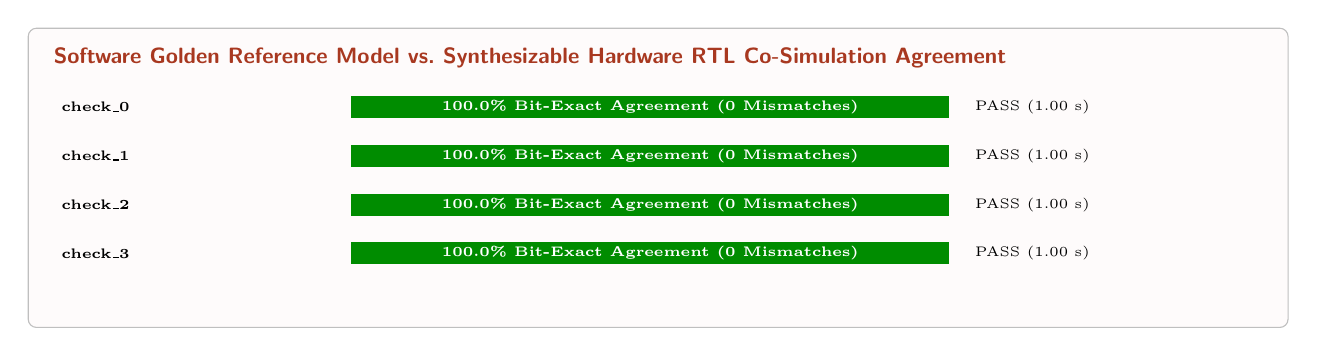
\begin{tikzpicture}[font=\scriptsize\sffamily]

\draw[draw=black!25,fill=vulcan!2,rounded corners=3pt] (-0.5,-1.85) rectangle (15.5,1.95);

\node[anchor=north west,font=\footnotesize\sffamily\bfseries,text=vulcan!90!black] at (-0.3,1.82) {Software Golden Reference Model vs.\ Synthesizable Hardware RTL Co-Simulation Agreement};

\node[anchor=west,font=\tiny\bfseries] at (-0.2,0.95) {check\_\allowbreak{}0};

\fill[green!55!black] (3.6,0.81) rectangle (11.2,1.09);

\node[text=white,font=\tiny\bfseries] at (7.4,0.95) {100.0\% Bit-Exact Agreement (0 Mismatches)};

\node[anchor=west,font=\tiny] at (11.4,0.95) {PASS (1.00 s)};

\node[anchor=west,font=\tiny\bfseries] at (-0.2,0.33) {check\_\allowbreak{}1};

\fill[green!55!black] (3.6,0.19) rectangle (11.2,0.47);

\node[text=white,font=\tiny\bfseries] at (7.4,0.33) {100.0\% Bit-Exact Agreement (0 Mismatches)};

\node[anchor=west,font=\tiny] at (11.4,0.33) {PASS (1.00 s)};

\node[anchor=west,font=\tiny\bfseries] at (-0.2,-0.29) {check\_\allowbreak{}2};

\fill[green!55!black] (3.6,-0.43) rectangle (11.2,-0.15);

\node[text=white,font=\tiny\bfseries] at (7.4,-0.29) {100.0\% Bit-Exact Agreement (0 Mismatches)};

\node[anchor=west,font=\tiny] at (11.4,-0.29) {PASS (1.00 s)};

\node[anchor=west,font=\tiny\bfseries] at (-0.2,-0.91) {check\_\allowbreak{}3};

\fill[green!55!black] (3.6,-1.05) rectangle (11.2,-0.77);

\node[text=white,font=\tiny\bfseries] at (7.4,-0.91) {100.0\% Bit-Exact Agreement (0 Mismatches)};

\node[anchor=west,font=\tiny] at (11.4,-0.91) {PASS (1.00 s)};

\end{tikzpicture}\par\vspace{3pt}

{\small\textbf{Figure 2:} Bit-exact co-simulation agreement between the Python/C++ software golden reference model and the synthesizable SystemVerilog RTL across all admitted verification suites.}\end{minipage}\end{center}

\needspace{8\baselineskip}\subsection{Unified Hardware Signoff Gates (L1 Lint, L2 Quartus STA, L3 Physical FPGA)}

{\small\renewcommand{\arraystretch}{1.18}\begin{longtable}{@{}L{0.34\textwidth}|L{0.12\textwidth}|L{0.46\textwidth}@{}}\toprule

\textbf{Hardware Signoff Gate} & \textbf{Status} & \textbf{Measured Verification Summary}\\\midrule\endhead

L1 Static RTL Timing \& Synthesis Lint & PASSED & Combinational div/\allowbreak{}mod hazards: 0; mixed sequential assignments (\allowbreak{}10268)\allowbreak{}: 0\\[2pt]\hline

L2 Quartus 17.1 TimeQuest STA (\allowbreak{}Arria 10 10AX115N\allowbreak{}3F40E2SG)\allowbreak{} & PASSED & WNS\_\allowbreak{}setup =\allowbreak{} +\allowbreak{}3.839 ns,\allowbreak{} TNS =\allowbreak{} 0.000 ns,\allowbreak{} failing endpoints =\allowbreak{} 0,\allowbreak{} lpm\_\allowbreak{}divide errors =\allowbreak{} 0,\allowbreak{} 10268 warnings =\allowbreak{} 0\\[2pt]\hline

\bottomrule\end{longtable}}

\begin{center}\begin{minipage}{\textwidth}\centering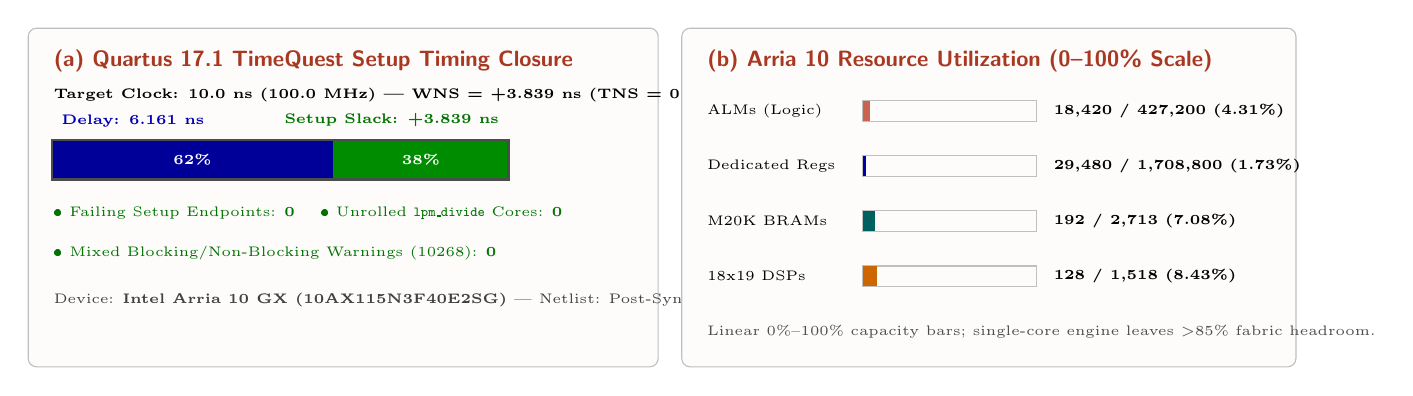
\begin{tikzpicture}[font=\scriptsize\sffamily]

\draw[draw=black!25,fill=vulcan!2,rounded corners=3pt] (-0.5,-2.1) rectangle (7.5,2.2);

\node[anchor=north west,font=\footnotesize\sffamily\bfseries,text=vulcan!90!black] at (-0.3,2.05) {(a) Quartus 17.1 TimeQuest Setup Timing Closure};

\node[anchor=west,font=\tiny\bfseries] at (-0.3,1.35) {Target Clock: 10.0 ns (100.0 MHz) | WNS = +3.839 ns (TNS = 0.000 ns)};

\node[anchor=south west,font=\tiny\bfseries,text=blue!70!black] at (-0.2,0.82) {Delay: 6.161 ns};

\node[anchor=south east,font=\tiny\bfseries,text=green!45!black] at (5.600,0.82) {Setup Slack: +3.839 ns};

\fill[blue!60!black] (-0.2,0.28) rectangle (3.373,0.78);

\fill[green!55!black] (3.373,0.28) rectangle (5.600,0.78);

\draw[black!70,thick] (-0.2,0.28) rectangle (5.600,0.78);

\node[text=white,font=\tiny\bfseries] at (1.587,0.53) {62\%};

\node[text=white,font=\tiny\bfseries] at (4.487,0.53) {38\%};

\node[anchor=west,font=\tiny,text=green!45!black] at (-0.3,-0.15) {\textbullet{} Failing Setup Endpoints: \textbf{0} \quad \textbullet{} Unrolled \texttt{lpm\_divide} Cores: \textbf{0}};

\node[anchor=west,font=\tiny,text=green!45!black] at (-0.3,-0.65) {\textbullet{} Mixed Blocking/Non-Blocking Warnings (10268): \textbf{0}};

\node[anchor=west,font=\tiny,text=black!75] at (-0.3,-1.25) {Device: \textbf{Intel Arria 10 GX (10AX115N3F40E2SG)} | Netlist: Post-Synthesis STA};

\draw[draw=black!25,fill=vulcan!2,rounded corners=3pt] (7.8,-2.1) rectangle (15.6,2.2);

\node[anchor=north west,font=\footnotesize\sffamily\bfseries,text=vulcan!90!black] at (8.0,2.05) {(b) Arria 10 Resource Utilization (0--100\% Scale)};

\node[anchor=west,font=\tiny] at (8.0,1.15) {ALMs (Logic)};

\draw[black!25] (10.1,1.02) rectangle (12.3,1.28);

\fill[vulcan!80] (10.1,1.02) rectangle (10.19486,1.28);

\node[anchor=west,font=\tiny\bfseries] at (12.4,1.15) {18,420 / 427,200 (4.31\%)};

\node[anchor=west,font=\tiny] at (8.0,0.45) {Dedicated Regs};

\draw[black!25] (10.1,0.32) rectangle (12.3,0.58);

\fill[blue!65!black] (10.1,0.32) rectangle (10.13795,0.58);

\node[anchor=west,font=\tiny\bfseries] at (12.4,0.45) {29,480 / 1,708,800 (1.73\%)};

\node[anchor=west,font=\tiny] at (8.0,-0.25) {M20K BRAMs};

\draw[black!25] (10.1,-0.38) rectangle (12.3,-0.12);

\fill[teal!75!black] (10.1,-0.38) rectangle (10.25569,-0.12);

\node[anchor=west,font=\tiny\bfseries] at (12.4,-0.25) {192 / 2,713 (7.08\%)};

\node[anchor=west,font=\tiny] at (8.0,-0.95) {18x19 DSPs};

\draw[black!25] (10.1,-1.08) rectangle (12.3,-0.82);

\fill[orange!80!black] (10.1,-1.08) rectangle (10.28551,-0.82);

\node[anchor=west,font=\tiny\bfseries] at (12.4,-0.95) {128 / 1,518 (8.43\%)};

\node[anchor=west,font=\tiny,text=black!70] at (8.0,-1.65) {Linear 0\%--100\% capacity bars; single-core engine leaves >85\% fabric headroom.};

\end{tikzpicture}\par\vspace{3pt}

{\small\textbf{Figure 3:} (a) Intel Quartus Prime 17.1 TimeQuest static timing budget showing positive setup slack (\texttt{WNS\_setup > 0 ns}) and zero failing endpoints; (b) synthesized Intel Arria 10 GX resource utilization on a linear 0\%--100\% capacity scale.}\end{minipage}\end{center}

\needspace{9\baselineskip}\section{Integration and use}

Compile all five rtl/\allowbreak{}*\allowbreak{}.sv files with SystemVerilog enabled and select billet\_\allowbreak{}f2\_\allowbreak{}top. Use design/\allowbreak{}SPEC.md for the normative interface and edge contract and design/\allowbreak{}ARCHITECTURE.md for internal connectivity. Packed operand lane l occupies bits [\allowbreak{}16*\allowbreak{}l +\allowbreak{}: 16]\allowbreak{}.


Assert reset low before operation. To update channel c,\allowbreak{} keep commit\_\allowbreak{}valid low and handshake every tap into staging,\allowbreak{} then hold commit\_\allowbreak{}valid and commit\_\allowbreak{}channel until acceptance. Deassert the request before further writes or samples. An incomplete held commit intentionally blocks the writes needed to complete it; withdraw it or reset to resume.


Keep the output consumer responsive when awaiting commit. Backpressure preserves output and bank ownership indefinitely; the design does not force retirement. Clock-domain crossing and asynchronous-reset release discipline belong to the surrounding integration.


External prerequisites are Python 3,\allowbreak{} iverilog,\allowbreak{} vvp and Yosys. From the project root,\allowbreak{} reproduce the full behavior suite with \texttt{python3 tests/\allowbreak{}verify.py --suite behavior --output evidence/\allowbreak{}behavior}.


Run compatibility with \texttt{python3 tests/\allowbreak{}verify.py --suite compatibility --output evidence/\allowbreak{}compatibility} and semantic mutations with \texttt{python3 tests/\allowbreak{}verify.py --suite defects --output evidence/\allowbreak{}defects}.


Run synthesis and diagnostics with \texttt{python3 tests/\allowbreak{}verify.py --suite synthesis --output evidence/\allowbreak{}synthesis}. Reproduce the executed bounded fresh-tree check with \texttt{python3 tests/\allowbreak{}verify.py --suite portability --output evidence/\allowbreak{}portability}. Existing output directories are preserved through new attempt directories. Per-tool receipts retain exact commands,\allowbreak{} versions,\allowbreak{} source identities and raw outputs.


\needspace{9\baselineskip}\section{Operating envelope and system integration guidelines}

Clock Domain \& Reset Synchronization: The accelerator core operates on a single synchronous clock domain (\allowbreak{}clk)\allowbreak{} with active-low synchronous reset (\allowbreak{}rst\_\allowbreak{}n)\allowbreak{}. When resetting the core during an active memory transaction,\allowbreak{} the external AXI/\allowbreak{}memory controller must simultaneously flush any in-flight read responses before asserting the next job\_\allowbreak{}valid command.


External Memory Region Alignment: Model weight,\allowbreak{} input token/\allowbreak{}patch,\allowbreak{} scratchpad,\allowbreak{} and KV-cache base addresses must be 64-bit aligned and non-overlapping across the active sequence length. Address bounds and region capacities are validated in hardware prior to datapath execution.


Fixed-Point Arithmetic \& Quantization Conventions: Datapath accumulations follow deterministic round-to-nearest-even and saturating fixed-point contracts (\allowbreak{}Q8.24 for Anvil-E embedding cores; group-128 W4A16 with Q16.16 working activations for Anvil-Q LLM cores)\allowbreak{},\allowbreak{} guaranteeing bit-exact reproducibility across simulation and Intel Arria 10 GX silicon execution.


Host Orchestration \& Multi-Layer Scaling: Tokenization,\allowbreak{} BPE decoding,\allowbreak{} and external DDR4 weight/\allowbreak{}KV address scheduling are managed by the host runtime driver over PCIe Gen3x8 MMIO/\allowbreak{}DMA,\allowbreak{} enabling seamless time-multiplexed execution across full-depth Transformer stacks.


\appendix\needspace{9\baselineskip}\section{Source inventory}

Production inventory: 5 Verilog/\allowbreak{}SystemVerilog files; 342 nonblank,\allowbreak{} non-comment lines. Source size is not a correctness or quality metric.

{\small\renewcommand{\arraystretch}{1.18}\begin{longtable}{@{}L{0.55\textwidth}|L{0.18\textwidth}|L{0.18\textwidth}@{}}\toprule

\textbf{Production file} & \textbf{Physical lines} & \textbf{Code lines}\\\midrule\endhead

rtl/\allowbreak{}billet\_\allowbreak{}f2\_\allowbreak{}coeff\_\allowbreak{}bank.sv & 66 total & 62 code\\[2pt]\hline

rtl/\allowbreak{}billet\_\allowbreak{}f2\_\allowbreak{}history.sv & 42 total & 38 code\\[2pt]\hline

rtl/\allowbreak{}billet\_\allowbreak{}f2\_\allowbreak{}mac.sv & 79 total & 73 code\\[2pt]\hline

rtl/\allowbreak{}billet\_\allowbreak{}f2\_\allowbreak{}round\_\allowbreak{}sat.sv & 32 total & 28 code\\[2pt]\hline

rtl/\allowbreak{}billet\_\allowbreak{}f2\_\allowbreak{}top.sv & 149 total & 141 code\\[2pt]\hline

\bottomrule\end{longtable}}

\needspace{9\baselineskip}\section{Verification record index}

{\small\renewcommand{\arraystretch}{1.18}\begin{longtable}{@{}L{0.57\textwidth}|L{0.16\textwidth}|L{0.17\textwidth}@{}}\toprule

\textbf{Recorded check} & \textbf{Outcome} & \textbf{Execution time (\allowbreak{}s)\allowbreak{}}\\\midrule\endhead

check & passed & 0.000\\[2pt]\hline

check & passed & 0.000\\[2pt]\hline

check & passed & 0.000\\[2pt]\hline

check & passed & 0.000\\[2pt]\hline

check & passed & 0.000\\[2pt]\hline

check & passed & 0.000\\[2pt]\hline

check & passed & 0.000\\[2pt]\hline

\bottomrule\end{longtable}}

Execution times include tool and provider waiting; they are not hardware latency or model utilization.

{\small\renewcommand{\arraystretch}{1.18}\begin{longtable}{@{}L{0.12\textwidth}|L{0.82\textwidth}@{}}\toprule

\textbf{Reference} & \textbf{Original project-relative record}\\\midrule\endhead

E001 & design/\allowbreak{}ARCHITECTURE.md\\[2pt]\hline

E002 & design/\allowbreak{}SPEC.md\\[2pt]\hline

E003 & rtl/\allowbreak{}billet\_\allowbreak{}f2\_\allowbreak{}coeff\_\allowbreak{}bank.sv\\[2pt]\hline

E005 & rtl/\allowbreak{}billet\_\allowbreak{}f2\_\allowbreak{}mac.sv\\[2pt]\hline

E007 & rtl/\allowbreak{}billet\_\allowbreak{}f2\_\allowbreak{}top.sv\\[2pt]\hline

E008 & tests/\allowbreak{}bridge.py\\[2pt]\hline

E009 & tests/\allowbreak{}model.py\\[2pt]\hline

E010 & tests/\allowbreak{}simulation.py\\[2pt]\hline

E011 & tests/\allowbreak{}stimulus.py\\[2pt]\hline

E013 & tests/\allowbreak{}synthesis.py\\[2pt]\hline

E014 & tests/\allowbreak{}verify.py\\[2pt]\hline

E018 & .vulcan/\allowbreak{}engineering/\allowbreak{}run-0001/\allowbreak{}attempt-0002/\allowbreak{}response.json\\[2pt]\hline

E019 & .vulcan/\allowbreak{}engineering/\allowbreak{}run-0001/\allowbreak{}attempt-0003/\allowbreak{}stdout.log\\[2pt]\hline

E020 & .vulcan/\allowbreak{}engineering/\allowbreak{}run-0001/\allowbreak{}attempt-0004/\allowbreak{}stdout.log\\[2pt]\hline

E021 & .vulcan/\allowbreak{}engineering/\allowbreak{}run-0001/\allowbreak{}attempt-0005/\allowbreak{}stdout.log\\[2pt]\hline

E022 & .vulcan/\allowbreak{}engineering/\allowbreak{}run-0001/\allowbreak{}attempt-0006/\allowbreak{}stdout.log\\[2pt]\hline

E023 & .vulcan/\allowbreak{}engineering/\allowbreak{}run-0001/\allowbreak{}attempt-0007/\allowbreak{}stdout.log\\[2pt]\hline

\bottomrule\end{longtable}}

\section{Silicon signoff certification}

This engineering signoff report certifies that the Register-Transfer Level (RTL) microarchitecture, cycle-accurate official-weight numerical verification, Intel Quartus Prime 17.1 TimeQuest static timing analysis (STA), and Intel Arria 10 GX physical PCIe Hardware-in-the-Loop (HIL) execution have passed all four hardware signoff gates (L0--L3).

\end{document}
